\documentclass[10pt,twocolumn,letterpaper]{article}

\usepackage{cvpr}
\usepackage{times}
\usepackage{epsfig}
\usepackage{graphicx}
\usepackage{amsmath}
\usepackage{amssymb}

% Include other packages here, before hyperref.

% If you comment hyperref and then uncomment it, you should delete
% egpaper.aux before re-running latex.  (Or just hit 'q' on the first latex
% run, let it finish, and you should be clear).
\usepackage[breaklinks=true,bookmarks=false]{hyperref}

\cvprfinalcopy % *** Uncomment this line for the final submission

\def\cvprPaperID{MLCV Project 2017} % *** Enter the CVPR Paper ID here
\def\httilde{\mbox{\tt\raisebox{-.5ex}{\symbol{126}}}}

% Pages are numbered in submission mode, and unnumbered in camera-ready
%\ifcvprfinal\pagestyle{empty}\fi
% \setcounter{page}{4321}

\begin{document}

%%%%%%%%% TITLE
\title{Cutting Constraints on Conservation Tracking\\
  \large{Project Report MLCV Summer 2017}
}

\author{Kodai Matsuoka\\
{\tt\small kodaig06@gmail.com}
\and
Yuyan Li\\
{\tt\small yuyan.li@gmx.net}
\and
Jui-Hung Yuan\\
{\tt\small j.yuan@stud.uni-heidelberg.de}
}

\maketitle
%\thispagestyle{empty}

%%%%%%%%% ABSTRACT
\begin{abstract}
\end{abstract}

%%%%%%%%% BODY TEXT
\section{Introduction}

To understand the complex biological functions of living organisms, many experiments require monitoring of stem cells or bacteria over several generations under different conditions. However, those time-lapse experiments generate large amount of data, which human observers could hardly analyze without bias. Thus, automatated systems for cell tracking are necessary for those studies.

The analysis of the time-lapse microscopic results usually requires not only the tracking of position and locomotion of individual cells, but also the reconstruction of their full lineage. In comparison to pedestrian tracking, the cell tracking task is more challenging due to the constant change of the cellular texture and morphology throughout the cell cycle, the high density of cells with uncertain movement as well as the division events which is not included in other multi-object tracking tasks.

To tackle the cell tracking task, a two-step pipeline consisting of a segmentation/detection phase and an assignment/tracking phase is commonly used. In the first phase, the raw input images are segmented into foreground and background. Those segmentations and the raw data are then fed into classifiers that generate the corresponding detection and division hypotheses. Using the outputs of the classifiers as potentials, a graphical model is built for all possible assignments of  detection hypotheses between time frames in the second phase. Such tracking approaches are known as \textit{Tracking-by-assignment} methods, which assume that the previous extracted set of detection hypotheses are over-complete and the constructed model thus describe all tracked targets. A globally consistent tracking solution is then reached via various optimization strategies.

The drawback of such method is that the errors in the first stage would propagate to, and warp, the tracking result. Such errors would occur where a cluster of objects is incorrectly represented by a single segment, termed as \textit{mergers} in this paper. To correct these over- and undersegmentation errors, the Conservation Tracking model which explicitly include the global consistency constraints was developed and was shown to outperform other tracking methods. From previous works, the Conservation Tracking model could be further reformulated into a constrained network flow problem which led to a tight LP relaxation and thus could be solved faster. Even without the constraints for divisions and mergers, the LP relaxation of the model that accounts for flow conservation would still yield integral solutions.

In this paper, we hence developed a iterative method that solve the problem with only the violated constraints identified in each iteration. (a bit more blablabla)


\section{Constrained Network Flow Reformulation of Consveration Tracking}


\subsection{Conservation Tracking Model}

\begin{figure}[t]
\begin{center}
\centering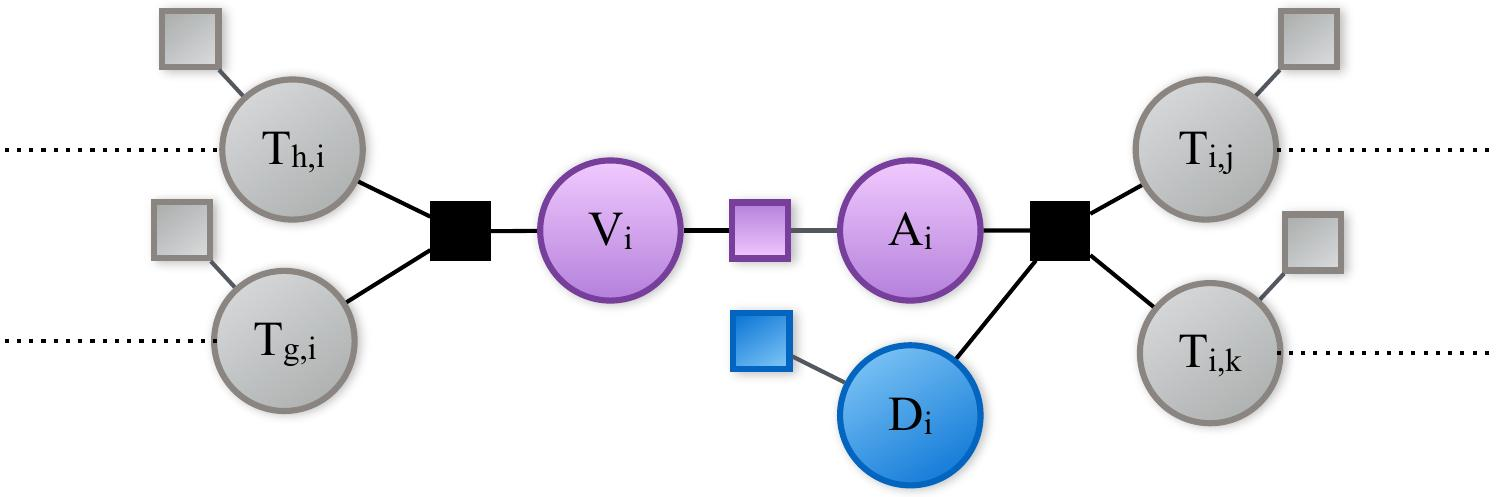
\includegraphics[width=0.8\linewidth]{model.jpeg}
\end{center}
   \caption{Factor graph for one detection with two incoming and two outgoing transition candidates. The circular nodes represent random variables, the non-black boxes describe factors that are dependent on the connected variables, and filled black boxes represent constraints. The purple detection node $i$ is seperated into a disappearance variable $V_i$ and an appearance variable $A_i$. The binary variable $D_i$ indicates whether object $i$ is about to divide. The transition variables $T \in \{0,...,m\}$ indicates the number of objects that are linked between two detection hypotheses.}
\label{fig:ctmodel}
\end{figure}

The Conservation Tracking model is presented in factor graphs as in Fig. \ref{fig:ctmodel}. The model contains three types of variables: \textit{Detection} variables $X_i \in \mathcal{X}$ (including the appearance $A_i \in \mathcal{A}$ and disappearance variables $V_i \in \mathcal{V}$) for each connected object from the segmented image, binary \textit{dividing} variables $D_i \in \mathcal{D}$ indicating whether an object is about to divide, and \textit{transition} variables $T_i \in \mathcal{T}$ that represent connections between the detections in two neighboring time frames. Noteworthy is that a division is allowed if and only if the corresponding detection contains one object. The probabilities of transition are modeled using the center of mass distance between detections, while the probabilities of appearance and disappearance are constant throughout time but linearly decrease to the edge of each image.

Let $\mathcal{Y}$ be the complete set of the configurations of all variables $\mathcal{V}\cup\mathcal{A}\cup\mathcal{T}\cup\mathcal{D}$, the approximate maximum a-posteriori (MAP) solution of the factor graph can be found by minimizing the energy
\scriptsize
\begin{equation*}
\begin{split}
 y^* &= \operatorname*{arg\,max}_{y\in\mathcal{Y}} E(y) \\ 
     &= \operatorname*{arg\,max}_{y\in\mathcal{Y}} \sum\limits_{V\in\mathcal{V}}\sum\limits_{A\in\mathcal{A}} E_x(y_V, y_A) + \sum\limits_{T\in\mathcal{T}} E_T(y_T) + \sum\limits_{D\in\mathcal{D}} E_D(y_D)
\end{split}
\end{equation*}
\normalsize
subject to constraints for flow conservation, division and mergers which will be explained in \ref{ILP formulation} in detail. This graphical model can be reformulated into a network flow and solved as an integer linear programming (ILP) problem.

\subsection{ILP for Network Flow}
\label{ILP formulation}
Linear Programming (LP) is a method to minimize (maximize) linear objective function, subject to linear inequality. Its formulation is as below.
\[
min_{x}  c^{T}x
\]
\[
s.t. Ax \leq b
\]
The objective function \(c^{T}x\) linearly depends on the vector \(x \in R^{n}\) which represents n variables in question. Constraint \(Ax \leq b\) defines n hyperplanes that disallow x to lie in the back side. The area where x satisfies all the constraints is called "polytope". It is proved that the optimal solution lies on a vertex of the polytope. For this reason, LP is solved in polynomial time by searching along vertices on the polytope.
When x takes only integer values (i.e. \(x \in Z^{n}\) ), the problem is called Integer Linear Programs (ILP). ILP is NP hard in general and cannot be solved in polynomial time. 
A common approach to solve ILPs is to ignore the integrarity constraints and to solve this relaxed LP. Since this "relaxed" problem is LP, we can solve it in polynomial time. From the solution, we gain the information about original ILP problem.
If the solution of relaxed LP is integtal - and hence coinsides with the solution of original ILP - , the relaxation is said to be "tight" around the optimum.


Network flow formulation.
Flownetwork is a directed graph with capacity on each edge. The flow can travel on directed graph under following rules. (1)The flow should not exceed the capacity. (2)The flow traveling to and from one node must be equal (Flow conservation). One can imagine as such networks water pipes, traffic network, electric circuits. There are several types of Network flow algorithms. For example, max-flow algorithm tries to maximize the flow from source to sink, and min-cost algorithm finds the route that minimize the cost. An important property here is that if all capacities are integers, optimal flow also takes an integer value. This situation corresponds to the constraint matrix(A) is totallly unimodular (TUM) in ILP, therefore LP relaxation is tight.

\begin{figure}[t]
\begin{center}
\centering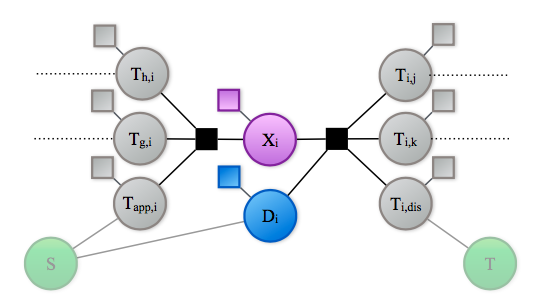
\includegraphics[width=0.8\linewidth]{model2.jpeg}
\end{center}
   \caption{Figure 2. In the constrained network flow graph, the detection node \(X_{i}\) is only a single node with unary factor, and appearances as well as disappearances are modeled as transitions \(T_{app,i}\) from an auxiliary source (green S ) or \(T_{i,dis}\) to an auxiliary sink (green T ) respectively.}
\end{figure}

We deal with the flow network graph as shown in Fig.2. Notation is slightly changed from 2.1, $X_i \in \mathcal{X}$ is \textit{Detection} variables and the appearance $A_i \in \mathcal{A}$ and disappearance variables $V_i \in \mathcal{V}$ are modeled in \textit{transition} variables. Every random variables $V \in \mathcal{V}$ take state $k \in \mathcal{L}(V) \equiv {0, ...,m}$ indicating the number of contained target, where m is the upper about on the number of targets that can be merged into one detection. We introduce a unary potential $\theta_{V}(k)$ for every random variables $V \in \mathcal{V}$. This is the negative lof of probability that V takes value k. The probability is givein by local observation.
Our formulation is as follows.

\begin{scriptsize}
\begin{equation*}
\begin{split}
 y^* &= \operatorname*{arg\,max}_{y\in\mathcal{Y}} E(y) \\ 
     &= \operatorname*{arg\,max}_{y\in\mathcal{Y}} \sum\limits_{X\in\mathcal{X}} E_X(y_X) + \sum\limits_{T\in\mathcal{T}} E_T(y_T) + \sum\limits_{D\in\mathcal{D}} E_D(y_D) \\
     &= \operatorname*{arg\,max}_{y\in\mathcal{Y}} \sum\limits_{X\in\mathcal{X}} \sum\limits_{k\in\mathcal{L(X)}} \theta_X(k) 1[y_X = k] + \sum\limits_{T\in\mathcal{T}} \sum\limits_{k\in\mathcal{L(T)}} 1[y_T = k] \newline \\
     & + \sum\limits_{D\in\mathcal{D}} \sum\limits_{k\in\mathcal{L(D)}} 1[y_D = k] 
\end{split}
\end{equation*}

subject to

Flow conservarion:
\[
\forall X\in\mathcal{X} \cup Sink : y_{X} = \sum\limits_{I\in\mathcal{I}(X)}y_{I}, 
\]
\[
\forall X\in\mathcal{X} \cup Source : y_{X} + Y_{D(X)} = \sum\limits_{O\in\mathcal{O}(X)}y_{O}
\]

Division:
\[
\forall D\in\mathcal{D} : y_{D} - y_{X(D)} \leq 0
\]

Merger:
\[
\forall X\in\mathcal{X}, \forall I\in\mathcal{I}(X),I \neq App(X) : 1[y_{I}=0]+1[y_{App(X)}=0] \geq 1
\]
\[
\forall X\in\mathcal{X}, \forall O\in\mathcal{O}(X),O \neq Dis(X) : 1[y_{O}=0]+1[y_{Dis(O)}=0] \geq 1
\]
\end{scriptsize}

where $\mathcal{I}(X)$ is incoming to X, $\mathcal{O}(X)$ is outgoing. The meaning of each constraint is
flow conservation :the number of incoming and out going are the same.
division constraint :one cell can dicide into at most two cells.
merger constraint :mergers cannot partially disappear.

Because of these additional constraints, the TUM property collapses, so LP relaxation is not tight.
Therefore, we will first solve without division and meger constraints and then add only violated constraints.
\subsection{Loosening Constraints}

On this we do cutting constraints! Because TUM something.

What we do is cut all constraints and try to solve. If it's solved, great, if not, we add constraints to nodes with flow violation. Then solve again. Repeat until we find valid solution or no new violated nodes.

\section{Experiments and Results}

Our models are: Drosophila and Rapoport (with and without mergers?)

\subsection{Solutions}

\subsection{Computation Time}


\section{Conclusion}

It works but isn't really worth it.


{\small
\bibliographystyle{ieee}
\bibliography{egbib}
}

\end{document}
